\documentclass[12pt]{extarticle}

\usepackage[T1]{fontenc}
\usepackage{polski}
\usepackage[utf8x]{inputenc}
\usepackage[polish]{babel}
\usepackage{url}
\usepackage{afterpage}

\usepackage[margin=1.3in]{geometry}
\usepackage{color}
\usepackage{graphicx}
\usepackage{float}
\usepackage{indentfirst}
\setlength\parindent{1cm}

\usepackage{listings}
\lstset{
	language=Java,
	basicstyle=\ttfamily,
	numbers=left,
 	numberstyle=\tiny,
	frame=tb,
	tabsize=4,
	columns=fixed,
	showstringspaces=false,
	showtabs=false,
	keepspaces,
	commentstyle=\color{red},
	keywordstyle=\color{blue}
}

\newtheorem{theorem}{Problem}

\begin{document}
\begin{titlepage}
    \begin{center}
        
\includegraphics[width=4cm]{polsl.png}\\[1cm]
        \textsc{\LARGE{Politechnika Śląska}}\\[0.5cm]
        \textsc{\LARGE{Wydział Automatyki, Elektroniki i~Informatyki}}\\[0.5cm]
        \textsc{\LARGE{Kierunek Informatyka}}\\[2.5cm]
        \LARGE{Praca magisterska}\\[1cm]
        \begingroup
            \fontsize{14pt}{17pt}\selectfont
            Analiza porównawcza przetwarzania strumieniowego w Java 8 \\ i realizacji zapytań SQL w pamięci
        \endgroup
    \end{center}
    \vspace{2cm}
    \begingroup
        \fontsize{14pt}{17pt}\selectfont
        \textbf{Autor:} Aleksander Grzybowski\\
        \textbf{Kierujący pracą:} dr inż. Ewa Płuciennik\\
    \endgroup

    \vspace{2.0cm}
    \begingroup
        \fontsize{12pt}{14pt}\selectfont
        \begin{center}
        Gliwice, kwiecień 2017
        \end{center}
    \endgroup
\end{titlepage}

\clearpage

\tableofcontents

\newpage

\section{Wstęp}

    TBD

\section{Bazy SQL in-memory}

\subsection{Zastosowanie}

    Bazy danych SQL są powszechnie stosowanymi rozwiązaniami do gromadzenia i odczytu danych. Struktura danych ściśle określona przez definicje tabel, ochrona integralności poprzez ograniczenia i więzy referencyjne oraz wygodny język SQL zachęcają do ich stosowania zarówno dla małych, jak i dużych zbiorów danych. Mimo pojawienia się nowych technologii, takich jak bazy dokumentowe typu MongoDB czy bazy grafowe typu Neo4j, tradycyjne bazy relacyjne są wciąż najczęściej stosowanym w praktyce rozwiązaniem. Bazy danych działające całkowicie w pamięci RAM wykorzystywane są w dużych hurtowniach danych, gdzie szybkość ma pierwszorzędne znaczenie, a zwyczajowo stosowane rozwiązania (pamięć podręczna, cache na poziomie aplikacji) nie spełniają wymagań biznesowych.

      Bazy danych działające w pamięci RAM są wykorzystywane głównie podczas procesu wytwarzania oprogramowania, jako tymczasowe środowiska do testowania programów wymagających dowolnej bazy danych SQL. Typowe aplikacje, zwłaszcza internetowe, z reguły wymagają bazy danych, natomiast nie jest konieczne stosowanie tego samego rozwiązania przy tworzeniu oprogramowania co przy wdrożeniu. Dzięki wykorzystaniu bibliotek typu ORM (Object Relational Mapping) możliwe jest transparentne użycie dowolnej bazy, o ile aplikacja nie wykorzystuje specyficznych rozszerzeń języka SQL dostarczanych przez producentów (powszechnie akceptowaną praktyką jest unikanie wiązania się z konkretną implementacją SQL). Dzięki wykorzystaniu pamięci programu jako miejsca zapisu danych, nie jest konieczne tworzenie baz poza aplikacją, a zawartość tracona jest po zamknięciu programu.  Interfejs programistyczny JDBC jest wspierany przez wszystkie te rozwiązania, tak więc zarówno bazy dyskowe, jak i in-memory obsługuje się praktycznie w ten sam sposób. 

\subsection{Wybór implementacji}

    Jako iż porównanie baz danych i strumieni w Java 8 powinno być rzetelne, konieczne jest wybranie do badań baz in-memory działających w środowisku maszyny wirtualnej Javy. Dwoma najpopularniejszymi rozwiązaniami są H2 oraz HSQLDB. Są one powszechnie stosowane w szkieletach aplikacji, takich jak Spring czy Grails, wspomagając start nowego projektu bez ściśle określonego schematu bazy, która generowana jest przy każdym starcie aplikacji. Implementują one w zdecydowanej większości standard ANSI-SQL, jednakże pewne niewielkie braki nie powodują problemów w przypadku niniejszej pracy, ze względu na zastosowanie najbardziej podstawowych elementów języka SQL przy badaniu wydajności. 

\section{Strumienie w Java 8}

\subsection{Wstęp}

    Stream API jest wprowadzonym w wersji 8 Javy komponentem biblioteki standardowej, który pozwala na tworzenie tzw. strumieni. Strumień jest abstrakcyjną reprezentacją ciągu obiektów, które pochodzą z pewnego źródła. Zazwyczaj strumienie tworzone są na podstawie kolekcji, ale możliwe jest także generowanie obiektów w locie. Strumienie obsługują wykonywanie prostych i złożonych operacji filtrowania, sortowania, mapowania i grupowania, przy czym możliwe jest też samodzielne tworzenie obiektów przetwarzających dane (interfejs \texttt{Collector}). Należy mieć na uwadze, że wszystkie wykonane w ciągu operacje wykonywane są 'leniwie', to znaczy, żadna obróbka danych nie zachodzi przed wykonaniem tzw. operacji terminalnej. Wystąpienie operacji terminalnej powoduje łańcuchowe wykonanie się wszystkich operacji pośrednich.

    Cechą szczególną strumieni jest możliwość ich łatwego zrównoleglania, udostępniona programistom w postaci metody \texttt{Stream.parallelStream}. Wielowątkowe przetwarzanie danych jest dość złożonym zagadnieniem w Javie, wymagającym dużej wiedzy na temat działania maszyny wirtualnej (Java Memory Model) i szczególnej ostrożności przy blokowaniu zasobów. Jako iż strumienie definiowane są zwykle przez funkcje nie zmieniające stanu, dodanie elementu równoległości jest znacznie prostsze. Jednym z celów niniejszej pracy jest zbadanie, jaki wpływ na wydajność mogą mieć równoległe strumienie.

\subsection{Przykład}

    Fragment \ref{streamexample} prezentuje przykładowe użycie strumieni. Dostępna jest kolekcja \newline \texttt{Collection<Customer> customers}, która zawiera obiekty reprezentujące klientów. Każdy klient posiada pola danych, informujące między innymi o kraju jego pochodzenia oraz stanie konta (jest to część modelu danych TPC, który zostanie omówiony szczegółowiej w rozdziale \ref{tpc}). Metoda \texttt{stream} tworzy strumień obiektów typu \texttt{Customer}, na którym wywoływane są metody strumieniowe. Metoda \texttt{Stream.filter} przyjmuje obiekt funkcyjny typu \texttt{Predicate}, który określa, czy dany element powinien znaleźć się w wynikowym strumieniu. Warto zaznaczyć, że możliwe jest wykorzystanie dowolnego kodu języka Java - nie ma tutaj ograniczeń na konkretny zbiór funkcji, jak w przypadku języka SQL. Metoda \texttt{sorted} zwraca nowy strumień, posortowany według podanego klucza - domyślnie porównywane są bezpośrednio obiekty znajdujące się w strumieniu. W tym przypadku wykorzystany został wariant metody sortującej, wykorzystujący funkcję wyciągającą klucz sortowania z obiektu (tutaj - stan konta klienta). Na koniec wyniki zbierane są do listy typu \texttt{java.util.List}. 

\begin{lstlisting}[label=streamexample, caption=Przykładowe wykorzystanie Stream API]

List<Customer> canadiansSortedByBalance = customers.stream()
    .filter(customer -> Objects.equals(
        customer.nation.name,
        "CANADA"
    ))
    .sorted(Comparator.comparing(
        customer -> customer.acctbal
    ))
    .collect(toList());

\end{lstlisting}

\begin{figure}
\centering
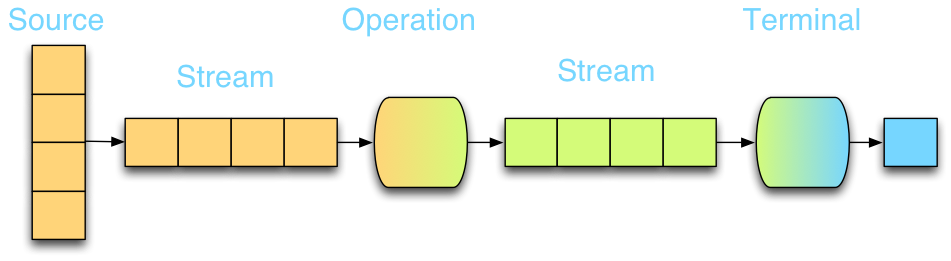
\includegraphics[width=14cm]{flow.png}
\caption{Przepływ danych}
\label{fig:flow}
\end{figure}

    Bardziej złożony przykład zaprezentowany jest na fragmencie \ref{advanced}. Kolekcja zamówień, na której opiera się zapytanie, składa się z obiektów typu \texttt{Order} posiadająch status oraz przyporządkowanego do zamówienia klienta. Podobnie jak w poprzednim przykładzie, w pierwszym kroku przeprowadza się filtrowanie jedynie zamówień o wyższym priorytecie. Następnie wykorzystana jest metoda \texttt{collect}, której zadaniem jest zebranie i przetworzenie wyników w ostateczną postać wynikową. Wykorzystano tutaj dwa zagnieżdżone kolektory, z których pierwszy dokonuje grupowania zamówień na podstawie przypisanego klienta, a drugi kolektor przejmuje pogrupowane zamówienia i dla każdej grupy określa ich wielkość, zliczając wszystkie obiekty w grupie. W ten sposób wyznaczone zostają liczby ważnych zamówień dla poszczególnych klientów.

\begin{lstlisting}[label=advanced, caption=Zaawansowane wykorzystanie Stream API]

List<String> high = asList("1-URGENT", "2-HIGH");
Map<Customer, Long> orderCountsByCustomer = orders.stream()
    .filter(o -> high.contains(o.orderPriority))
    .collect(
        Collectors.groupingBy(order -> order.customer,
            Collectors.counting()
        )
    );
    
    

\end{lstlisting}

\subsection{Biblioteka \texttt{ForkJoinPool}}

    Język Java od samego początku istnienia wyróżniał się znakomitymi możliwościami programowania równoległego, wykorzystywanego głównie w aplikacjach internetowych, obsługujących wielu użytkowników jednocześnie. Świadczy o tym obecność metod związanych z wątkami już w klasie \texttt{Object}, która jest klasą bazową wszystkich klas języka Java. W wersji 5 języka wprowadzono dużo nowych klas, zawartych w pakiecie \texttt{java.util.concurrent}, mających na celu ułatwienie pracy z równoległym kodem. Wcześniej ręcznie tworzone rozwiązania i wzorce mogą być zastąpione przez wbudowane, wysokiej jakości implementacje pul wątków, kolejek blokujących, list typu copy-on-write, semaforów i barier cyklicznych.
    
    Wersja siódma języka przyniosła kolejną nowość w postaci mechanizmu FJP, umożliwiającego uproszczone tworzenie równolegle wykonywanych framentów kodu, wykorzystujące bezpośrednio regułę "dziel i rządź". Tworzona jest pula wątków (o dowolnej ich ilości), do której wysyła się zadanie, będące obiektem klasy \texttt{RecursiveTask}. Klasa ta reprezentuje pojedyncze zadanie, które potrafi w razie potrzeby podzielić się na $ n $ mniejszych zadań. W kodzie programu należy sprawdzić, czy ten fakt występuje. Jeśli tak, zadanie należy podzielić, wysłać do puli wątków i zebrać wyniki po zakończeniu wykonywania się podzadań. W przeciwnym przypadku wystarczy zwrócić wynik. Przykładowy kod programu, mający na celu zsumowanie listy liczb całkowitych, zaprezentowany jest na fragmencie \ref{fjpexample}.

\begin{lstlisting}[label=fjpexample, caption=Przykładowe wykorzystanie FJP]

public class SummingTask extends RecursiveTask<Integer> {
  
  private List<Integer> source;
  
  SummingTask(List<Integer> source) {
    this.source = source;
  }
  
  @Override
  protected Integer compute() {
    if (source.size() > 1) {
      List<SummingTask> tasks = splitTasks();
      
      invokeAll(tasks);
      
      int partialSum = 0;
      for (SummingTask task : tasks) {
        partialSum += task.join();
      }
      return partialSum;
    } else {
      return source.get(0);
    }
  }
  
  private List<SummingTask> splitTasks() {
    return asList(
        new SummingTask(source.subList(
          0, source.size() / 2)
        ),
        new SummingTask(source.subList(
          source.size() / 2, source.size()
        )
      )
    );
  }
  
  public static void main(String[] args) {
    ForkJoinPool forkJoinPool = new ForkJoinPool(10);
    SummingTask task = new SummingTask(
      asList(1, 2, 3, 4, 5, 6, 7, 8, 9)
    );
    Integer sum = forkJoinPool.submit(task).get();
    System.out.println(sum);
  }
}

\end{lstlisting}

    FJP wykorzystany został przy implementacji równoległych strumieni. Jego znajomość nie jest konieczna do ich używania, natomiast może być przydatna przy badaniu wydajności przetwarzania strumieniowego. Domyślnie, przy tworzeniu strumienia nie jest możliwe wybranie puli wątków, w której przetwarzanie będzie zachodzić - przy bezpośrednim użyciu FJP jest to możliwe, wraz z określeniem docelowej, maksymalnej liczby wątków. Przeprowadzono dodatkowy eksperyment, w którym zbadano wydajność (liczbę operacji na sekundę) sortowania 1000000 liczb całkowitych, przy wykorzystaniu równoległych strumieni i zadania wykonywanego bezpośrednio w puli FJP, w zależności od liczby wątków puli. Kod źródłowy znajduje się w pliku \texttt{FJPSorting.java}, a rysunek \ref{fig:fjpsorting} prezentuje wyniki eksperymentu.

\begin{figure}[H]
\centering
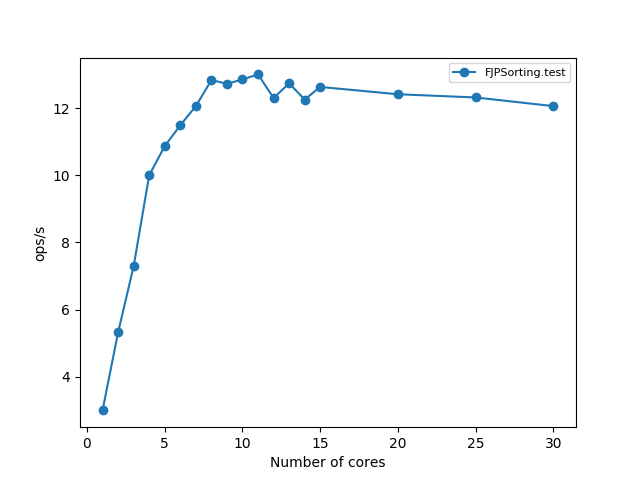
\includegraphics[width=13cm]{plots/FJPSorting}
\caption{Sortowanie 1000000 liczb w puli wątków FJP}
\label{fig:fjpsorting}
\end{figure}

    Jak można zauważyć, ilość operacji na sekundę rośnie przy wzroście wielkości puli do pewnego momentu, w którym narzut wielowątkowości staje się zbyt duży. Przyjęło się za ogólnie dobrą praktykę, aby liczba wątków była w przybliżeniu równa liczbie logicznych rdzeni procesora. Test przeprowadzono na maszynie z 4 rdzeniami Hyper Threading (logiczne 8 rdzeni), w związku z tym można się spodziewać optymalnego działania procesu dla takiej liczby wątków.




\subsection{Przetwarzanie równoległe i interfejs \texttt{Collector}}

    Jednym z najczęstszych zastosowań strumieni jest równoległe przetwarzanie danych. Strumienie równoległe wykorzystują FJP, natomiast w pełni enkapsulują jego wykorzystanie w taki sposób, że w większości przypadków wiedza na temat szczegółów implementacyjnych nie jest konieczna. Poszczególne zadania przetwarzania danych (filtrowanie, mapowanie itd.) wykonują się w tworzonej na starcie puli wątków, w której domyślnie znajduje się $ n-1 $ wątków, gdzie $ n $ jest liczbą logicznych rdzeni procesora. Najlepiej widać to na fragmencie \ref{streamsthreads}, w którym dla każdego elementu wypisywana jest nazwa wątku, w którym kod domknięcia jest wykonywany.  Wynikiem wywołania tego programu jest przemieszana lista wątków, w której znajdują się wątek główny programu \texttt{main} oraz wątki znajdujące się w puli o nazwach podobnych do \texttt{ForkJoinPool.commonPool-worker-3} z numerami od 1 do 7 (test przeprowadzony na maszynie z 8 logicznymi procesorami).

\begin{lstlisting}[label=streamsthreads, caption=Struktura puli wątków FJP]

IntStream.range(1, 100).parallel()
  .forEach(e -> out.println(
    Thread.currentThread().getName()
  )
);

\end{lstlisting}

    Interfejs \texttt{Collector} jest ważną częścią Stream API. Pozwala on na definiowanie tzw. operacji terminalnych, czyli takich, które mogą występować jedynie na samym końcu potoku przetwarzania strumieniowego. Jest to dość niskopoziomowy mechanizm, który jednak nie jest zbyt skomplikowany, a wymusza na programiście zwrócenie uwagi na przetwarzanie równoległe. Parametrem wejściowym obiektu kolektora jest strumień obiektów, przy czym nie jest on przekazywany jawnie, a poszczególne obiekty dostarczane są do odpowienich funkcji definujących kolektor. Wynikiem działania kolektora jest dowolny obiekt bądź kolekcja, ale w założeniu jest to wynik operacji redukującej strumień danych. Instancja kolektora nie posiada stanu - cały stan jest kontrolowany przez wewnętrzne struktury Stream API, co jest bardzo pożądane zwłaszcza w przypadku strumieni równoległych, w przypadku których zachowanie bezpieczeństwa wątkowego byłoby utrudnione

    Do utworzenia obiektu \texttt{Collector} wymagane są trzy (w szczególnym przypadku cztery) funkcje.

\begin{itemize}
    \item \texttt{Supplier<T> supplier} - funkcja tworząca pośredni kontener danych
    \item \texttt{BiConsumer<R, T> accumulator} - funkcja dodająca nowy element do pośredniego kontenera
    \item \texttt{BinaryOperator<R> combiner} - funkcja scalająca dwa pośrednie kontenery w jeden
    \item \texttt{Function<A, R> finisher} (opcjonalnie) - funkcja przekształcająca pośredni kontener danych w obiekt wynikowy
\end{itemize}

    Konieczność istnienia pośrednich kontenerów i możliwości ich scalania związana jest bezpośrednio z równoległą naturą strumieni. Jako iż kolektory powinny działać w identyczny sposób ze strumieniami sekwencyjnymi, jak i równoległymi, narzucony został wzorzec uwzględniający przetwarzanie równoległe w każdym przypadku.

    Fragment \ref{toList} prezentuje przykład ręcznie zaimplementowanego kolektora \texttt{toList}, który dostępny jest domyślnie w bibliotece standardowej języka Java. 

\begin{lstlisting}[label=toList, caption=Ręczna implementacja \texttt{toList}]

Collector<Integer, List<Integer>, List<Integer>> toList =
Collector.of(
    () -> {
      ArrayList<Integer> list = new ArrayList<>();
      out.println("New mutable container " + id(list));
      return list;
    },
    (acc, val) -> {
      out.println("Adding " + val + " to " + id(acc));
      acc.add(val);
    },
    (acc1, acc2) -> {
      out.println(
        "Combining " + id(acc1)
        + " with " + id(acc2)
      );
      acc1.addAll(acc2);
      return acc1;
    }
);

List<Integer> numbers = asList(1, 2, 3, 4, 5, 6, 7, 8, 9);

out.println(numbers.stream().collect(toList));

\end{lstlisting}

Wynik wykonania tego programu zaprezentowany jest na poniższym wyjściu programu. Warto zauważyć, że funkcja łącząca pośrednie kontenery nie została w ogóle wywołana. 
    
\begin{verbatim}

New mutable container #6b7
Adding 1 to #6b7
Adding 2 to #6b7
Adding 3 to #6b7
Adding 4 to #6b7
Adding 5 to #6b7
Adding 6 to #6b7
Adding 7 to #6b7
Adding 8 to #6b7
Adding 9 to #6b7
[1, 2, 3, 4, 5, 6, 7, 8, 9]

\end{verbatim}

Przy wykorzystaniu strumieni równoległych, wynik prezentuje się zupełnie inaczej. Tworzona jest duża ilość kontenerów pośrednich, a wszystkie operacje dodawania i łączenia wykonywane są równolegle w osobnych wątkach.

\begin{verbatim}

New mutable container #42c
New mutable container #678
Adding 1 to #42c
New mutable container #2d8
New mutable container #1e6
New mutable container #1df
New mutable container #37c
New mutable container #585
New mutable container #51f
Adding 2 to #585
Adding 7 to #37c
Adding 3 to #1df
Adding 6 to #1e6
New mutable container #46f
Adding 4 to #2d8
Combining #1df with #2d8
Adding 5 to #46f
Adding 9 to #678
Combining #46f with #1e6
Combining #42c with #585
Adding 8 to #51f
Combining #42c with #1df
Combining #51f with #678
Combining #37c with #51f
Combining #46f with #37c
Combining #42c with #46f
[1, 2, 3, 4, 5, 6, 7, 8, 9]

\end{verbatim}

    Automatyczny podział pierwotnego zadania na zadania mniejsze, wykonanie ich, oraz ich późniejsze scalenie odbywa się w całości w wewnętrznym kodzie Stream API. Podany przykład jest przykładem znacznie uproszczonym. Możliwe jest wykonywanie bardzo złożonych operacji na danych (np. zbieranie statystyk), o ile możliwy jest podział i scalenie zadań.

\section{Różnice pomiędzy metodami}

    Pomiędzy przetwarzaniem strumieniowym, a bazami SQL działającymi w pamięci występuje bardzo dużo różnic, pomimo pozornie podobnej zasady działania i efektu końcowego. Celem obu podejść jest uzyskanie wygodnego i względnie szybkiego wykonywania zapytań, natomiast różnice w implementacji znacząco wpływają na ten cel.

\subsection{Struktury danych}

    Głównym blokiem budującym w modelu relacyjnej bazy danych jest relacja (tabela) posiadająca kolumny i rekordy, a integralność danych zapewniona jest w pewnym stopniu przez ograniczenia, klucze i więzy referencyjne. Język SQL pozwala dzięki mechanizmowi JOIN na łatwe łączenie powiązanych ze sobą tabel i uzyskiwanie połączonych wyników. Jeśli baza danych została odpowienio zaprojektowana, uwzględniając wymaganą normalizację danych, to łączenie tabel na podstawie kluczy obcych jest naturalne dla programisty i proste w zrozumieniu. W przetwarzaniu strumieniowym pojęcie tabeli nie istnieje, ponieważ kontenerami danych są zwykłe kolekcje języka Java (listy, zbiory i mapy). O ile istnieją biblioteki bazodanowe typu jOOQ, które pozwalają na konwersję wyniku zapytania JDBC na strumień, to tak naprawdę operacje strumieniowe wykonują się zawsze na kolekcji w pamięci maszyny wirtualnej. W związku, aby operacje strumieniowe były wygodne dla programisty, model danych powinien uwzględniać powiązania między poszczególnymi obiektami w typowy dla języka Java sposób, poprzez referencje do innych obiektów (kompozycja). Łączenie kolekcji, choć możliwe, komplikuje znacznie zapytania i zmniejsza ich ogólną szybkość.

    Bazy in-memory wykorzystują wewnątrz struktury danych, które są ścisłym szczegółem implementacyjnym, niewidocznym dla programisty i ukrytym przed zmianami. Jest to w większości przypadków dobre rozwiązanie, pozwalające na odseparowanie wewnętrznej reprezentacji danych od metody dostępu do nich (przykładowo, dane w bazie H2 reprezentowane są przez obiekty klas \texttt{org.h2.mvstore.Page} i \texttt{org.h2.value.*}). Jednakże przy takim podejściu programista nie ma możliwości optymalizacji (o ile to możliwe) struktur danych i musi polegać na wykorzystanym w silniku bazy optymalizatorze zapytań. W przypadku strumieni wewnętrzne procesy zachodzące przy przetwarzaniu danych są ukryte, natomiast możliwe jest w każdym przypadku przepisanie części procesu na czystą Javę. Strumienie są bardzo wydajne, natomiast tak jak każda abstrakcja nad danymi wprowadzają pewnien niewielki narzut. W przypadku, gdy szybkość jest parametrem krytycznym, możliwe jest zastąpienie operacji klasy \texttt{Stream} zwykłymi konstrukcjami języka (pętle, warunki). 

\subsection{Weryfikacja poprawności składni}

    Przy wykonywaniu zapytania SQL z poziomu API JDBC nie istnieje żadne sprawdzanie poprawniości zapytania oraz jego składni w czasie kompilacji. Zapytanie wysyłane jest jako zwykły ciąg znaków do serwera bazodanowego, który następnie odczytuje zapytanie i przystępuje do jego interpretacji i wykonania. W związku z tym niemożliwe jest zapewnienie, czy dana tabela istnieje, albo czy dana funkcja SQL istnieje w danym oprogramowaniu bazy danych. Istnieją co prawda rozwiązania typu ORM, które chronią programistę przed niewłaściwym wykorzystaniem obiektu odwzorowanego na tabelę, albo edytory programistyczne z integracjami z serwerami baz, które umożliwiają przeskanowanie istniejących symboli (nazw tabel, kolumn itp.) i skorygowanie programisty, natomiast są to rozwiązania zewnętrzne, działające poza językiem Java. Przetwarzanie strumieniowe odbywa się w całości w języku Java, który jest silnie typowany, przez co niewłaściwe wykorzystanie konstrukcji języka zostanie automatycznie dostrzeżone przez kompilator. Przykładowo, wynikiem grupowania zbioru obiektów typu \texttt{T} na podstawie ich pola o typie \texttt{U} będzie zawsze \texttt{Map<T, List<U>}\texttt{>}. Dzięki temu typowe błędy przy odczytywaniu wyników z zapytania SQL przy użyciu obiektu \texttt{ResultSet} (niewłaściwy typ kolumny, niestniejące pole) nie występują.

\subsection{Język domenowy (DSL) a język ogólnego przeznaczenia}

    Język SQL, poza metodami dostępu do danych umożliwia także ich wstępne przetwarzanie. Dostępne są proste funkcje matematyczne, funkcje operujące na ciągach znaków czy datach. Problemem jest jednak często brak standaryzacji - różni dostawcy baz danych rozszerzają możliwości języka o różne funkcje, przez co migracja pomiędzy bazami danych może być problematyczna, zwłaszcza, jeśli w użyciu są własne procedure składowane (stored procedures). Przy użyciu Stream możliwe jest wykorzystanie praktycznie dowolnego kodu Javy, przez co aplikacja je wykorzystująca jest znacznie bardziej przenośna i łatwiej testowalna.
    

\section{Środowisko badawcze}

\subsection{Kryteria oceny}

    W niniejszej pracy pod pojęciem 'wydajność' rozumie się efektywny, uśredniony czas wykonania się danego zapytania i uzyskania wyników dostępnych w pamięci programu. Kryterium czasowe zostało przyjęte ze względu na łatwość jego pomiaru i bezpośrednie jego przełożenie na ogólną wydajność systemu wykorzystującego dany system bazodanowy. Niemniej jednak, w celach porównawczych, wykonane zostały również pomiary ilości zajętej pamięci, w celu zbadania wpływu struktur danych baz in-memory na zużycie pamięci. Jednym z problemów może być działanie odśmiecacza (garbage collector), który może być uruchamiany przez maszynę wirtualną Java w różnych fazach wykonywania badań, tak więc konieczna jest szczególna ostrożność przy interpretowaniu wyników.
    Jedną z trudności, które napotkano przy wykonywaniu eksperymentów, jest znaczny wpływ zastosowanej platformy sprzętowej na uzyskane wyniki. Oczywiście wydajność procesora będzie różnicowała ilość operacji na sekundę, natomiast konieczne jest sprawdzenie, czy relatywne porównanie wyników na różnych platformach jest jest takie same. Jeśli tak, to możliwe jest wyciągnięcie bardziej ogólnych wniosków z uzyskanych wyników, w przeciwnym przypadku możliwe jest, że dobór platformy sprzętowej jest istotny.
    Przy porównywaniu dwóch zupełnie różnych metod dostępu do danych, konieczne jest ustalenie postaci wynikowej pojedynczego eksperymentu. W przypadku języka SQL i metod JDBC wynik zapytania do bazy danych reprezentowany jest przez obiekt \texttt{ResultSet}, który udostępnia metody do poruszania się po wynikowych wierszach i wyciągania pojedynczych kolumn. W przypadku Stream API, rezultat zapytania dostępny jest od razu w formie obiektów standardowych kolekcji języka Java, takich jak \texttt{List<T>} czy \texttt{Map<K,V>}. W związku z tym, aby zapewnić sprawiedliwe porównanie obu metod, po wykonaniu zapytania SQL konieczne jest rozpakowanie obiektu \texttt{ResultSet} i przeniesienie danych do kolekcji Javy, aby uzyskać wynik w tej samej postaci.

\subsection{Budowa środowiska badawczego}

    Aby zebrane wyniki były jak najbardziej miarodajne, konieczne jest utworzenie solidnego środowiska testowego, w którym możliwe będzie wykonanie wszystkich potrzebnych badań. Jako iż elementem badań wydajności będą fragmenty kodu, pożądane jest, by pomiary czasowe odbywały się w miarę możliwości w sposób zautomatyzowany, generując pod koniec szczegółowy raport.

    JMH (Java Microbenchmark Harness) jest najpopularniejszym narzędziem służącym do tzw. microbenchmarkingu, czyli badania wydajności czasowej krótkich fragmentów kodu. Typowe metody pomiaru czasu w kodzie maszyny wirtualnej Javy nie są dokładne ani odporne na błędy, przykładowo często stosowane wywołanie \texttt{System.currentTimeMillis} nie jest odporne na zmiany czasu systemowego w trakcie wykonywania badania i ma różną dokładność na różnych systemach operacyjnych, natomiast \texttt{System.nanoTime()} nie jest bezpieczna wątkowo na poziomie procesora, przez co wykonywanie się zadań testowych na kilku rdzeniach procesora może powodować mylące wyniki. Co więcej, ręczne wykonywanie pomiarów jest dość żmudne i wymagałoby stworzenia własnego narzędzia. Zdecydowano się więc na wykorzystanie narzędzia gotowego. Przy użyciu JMH możliwe jest proste definiowanie metod, których wydajność (wykonania na sekundę) będzie badana, możliwe jest określenie ilości iteracji, ustalanie zmienych parametrów (np. ilość wierszy danych testowych). Raport wynikowy zawiera szczegółowe informacje na temat ilości wykonań metody, wariancje czasów oraz inne statystyki, na podstawie których możliwe jest wyciągnięcie potrzebnych wniosków.

    Do budowania projektu wykorzystano Gradle, które jest popularnym i używanym w zastosowaniach produkcyjnych narzędziem budowania projektów w Javie. Służy ono do uruchamiania kompilacji, uruchamiania testów jednostkowych, jak i wykonywania testów wydajnościowych dzięki integracji z JMH, które dostępne jest w ekosystemie Gradle jako gotowy plugin z możliwością dowolnej konfiguracji.

\subsection{Schemat klasy testu referencyjnego (microbenchmark)}

\begin{lstlisting}[label=testclass, caption=Przykładowa klasa JMH]

@SuppressWarnings("SqlResolve")
@State(Scope.Thread)
public class SummingIntegersH2 {
  
  private Connection connection;
  
  @Param({"100", "1000", "10000"})
  public int numberCount;
  
  @Setup
  public void setup() throws Exception {
    connection = newDatabase("h2");
    connection.createStatement().execute(
        "CREATE TABLE numbers (val INT)"
    );
    Random random = new Random(12345L);
    
    for (int i = 0; i < numberCount; ++i) {
      int randomNumber = random.nextInt(1000);
      connection.createStatement()
          .execute(
              "insert into numbers values ("
                  + randomNumber +
                  ")"
          );
    }
  }
  
  @Benchmark
  public int sql() throws Exception {
    ResultSet resultSet = connection
        .createStatement()
        .executeQuery("SELECT sum(val) FROM numbers");
    resultSet.next();
    
    return resultSet.getInt(1);
  }
}


\end{lstlisting}

    Każdy zbiór metod testujących wydajność danego rozwiązania zawarty jest w jednej klasie testowej, której przykład zaprezentowany jest na fragmencie \ref{testclass}. Metoda \texttt{setup} przygotowuje potrzebne dane testowe - generując je w czasie wykonania programu w przypadku danych losowych, bądź wczytuje z plików w przypadku wykorzystania testu TPC. Dane testowe ładowane są do bazy SQL oraz do zwykłych kolekcji języka Java, głównie list. Pozostałe metody, oznaczone adnotacją \texttt{@Benchmark} są metodami przeznaczonymi do profilowania. Biblioteka JMH zapewnia dokładny pomiar czasu wykonywania się fragmentów kodu, chroni przed zbyt agresywnymi optymalizacjami maszyny wirtualnej oraz udostępnia wygodny raport z przeprowadzonych testów, wraz z danymi statystycznymi typu wariancja.

\section{Dane testowe i wyniki}

\subsection{Dane testowe syntetyczne}

    W celu zbadania, ile czasu zajmują proste operacje na danych, zaproponowano kilka przypadków testowych operujących na syntetycznych, pseudolosowych danych testowych. Zapytania dobrano w taki sposób, aby prezentowały typowe operacje filtrowania i grupowania, często spotykane w aplikacjach. Dane testowe generowane są przy użyciu standardowych mechanizmów Javy, przy wykorzystaniu stałego ziarna generatora pseudolosowego w celu zapewnienia powtarzalności wyników. Każdy eksperyment wykonywany był na wygenerowanym zbiorze testowym o odpowiedniej wielkości, w zależności od przypadku i możliwości sprzętowych.

\begin{itemize}
    \item \texttt{SummingIntegers} - obliczenie sumy liczb w kolumnie
    \item \texttt{GroupingAndSumming} - obliczenie sum liczb w kolumnie \texttt{val1} po uprzednim pogrupowaniu ich na podstawie kolumny \texttt{val2}
    \item \texttt{CrossJoinAndFilter} - złączenie naturalne
    \item \texttt{FilteringAndCountingIntegers} - wyszukanie dodatnich liczb oraz ich policzenie
    \item \texttt{HugeJoining} - iloczyn kartezjański dwóch kolumn
\end{itemize}


\subsection{Wyniki badań dla danych syntetycznych}

    Już po pobieżnym spojrzeniu na wyniki testów rzuca się w oczy kilka wniosków. Najszybszą i zarazem najprostszą ciągła strukturą danych jest zwykła tablica typu prymitywnego. Ze względu na zachowanie ciągłości w pamięci (w typowych implementacjach) i najszybszym możliwym czasie dostępu do elementów z bardzo niskim poziomem abstrakcji, proste operacje wymagające sekwencyjnego odczytu są najszybsze spośród porównanych. Czasy sumowania liczb w tablicy, w porównaniu do czasów sumowania liczb w liście są średnio 3x mniejsze. Należy jednak zaznaczyć, że optymalizacje tego typu znacząco utrudniają pisanie kodu, ze względu na rezygnację z wygodnych metod interfejsu \texttt{List<T>}. W większości typowych, biznesowych zastosowań mikrooptymalizacje tego typu nie będą istotne z punku widzenia wydajności całych aplikacji, aczkolwiek w pewnych szczególnych zastosowaniach (np. dziedzina High Frequency Trading) mogą mieć pewne znaczenie.

    W zbadanych przypadkach strumienie równoległe wykazują większą wydajność niż strumienie sekwencyjne od pewnego rozmiaru danych wejściowych. Utworzenie strumienia równoległego i jego skonsumowanie wymaga uruchomienie całego procesu podziału danych na wątki, wykonywania operacji i łączenia wyników z poszczególnych wątków. Daje to pewien narzut, który jest szczególnie widoczny przy małych listach, dla których operacje sekwencyjne wykonują się szybciej. Niestety, nie istnieje sposób pozwalający przewidzieć, który rodzaj strumienia (sekwencyjny czy równoległy) byłby lepszym wyborem dla danej sytuacji. Możliwe byłoby zaproponowanie heurystycznej metody, określającej rodzaj na podstawie wielkości danych wejściowych, ale nie byłby on niezawodny, więc dobór metody pozostawiony jest programiście.

    Strumienie i bezpośrednie operacje na pamięciowych strukturach języka Java są w zdecydowanej większości przypadków szybsze niż ich odpowiedniki w języku SQL. Porównując zaś bazy H2 i MySQL, testy na bazie H2 wykonywane było średnio 1.5-20x razy szybciej niż w przypadku MySQL. Związane jest to z pewnością w pewnym stopniu z narzutami transmisji i konwersji danych pomiędzy procesami. Do połączenia się z bazą dyskową wykorzystany został, tak jak w przypadku bazy pamięciowej, standardowy interfejs JDBC, który wykorzystywał połączenie TCP. Przepustowość tego połączenia nie powinna mieć zbytniego znaczenia (prędkość połączenia typu loopback determinowana jest głównie przez moc procesora, a ilość danych przesyłanych jest znikoma), większy wpływ ma złożoność systemu bazodanowego i metody składowania danych. Należy zauważyć, że w przypadku największych zbiorów testowych różnice w wydajności nie przekraczają 2-3x. Jest to z pewnością związane z przystosowaniem i optymalizacjami baz dyskowych.

\begin{figure}[H]
\centering
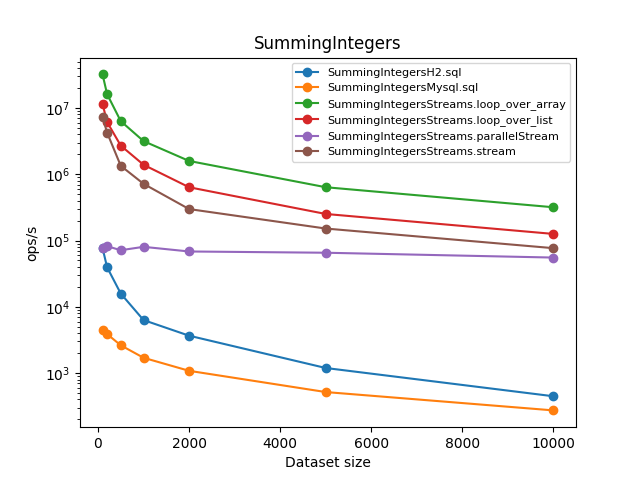
\includegraphics[width=13cm]{plots/SummingIntegers}
\caption{SummingIntegers}
\end{figure}

\begin{figure}[H]
\centering
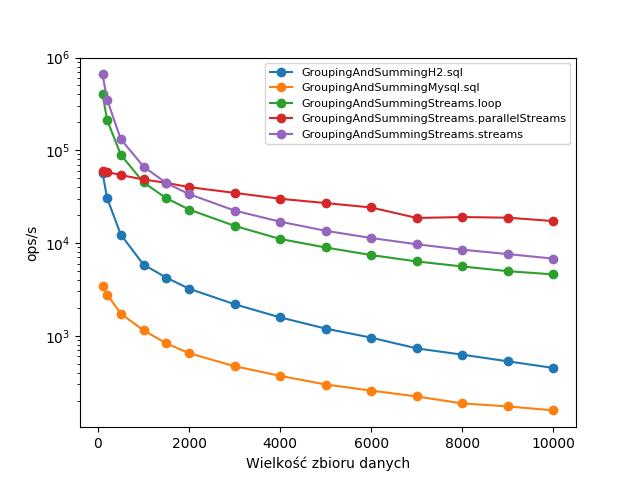
\includegraphics[width=13cm]{plots/GroupingAndSumming}
\caption{GroupingAndSumming}
\end{figure}

\begin{figure}[H]
\centering
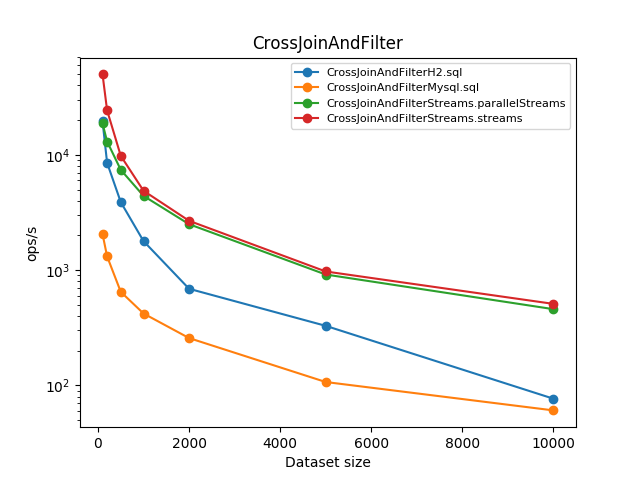
\includegraphics[width=13cm]{plots/CrossJoinAndFilter}
\caption{CrossJoinAndFilter}
\end{figure}

\begin{figure}[H]
\centering
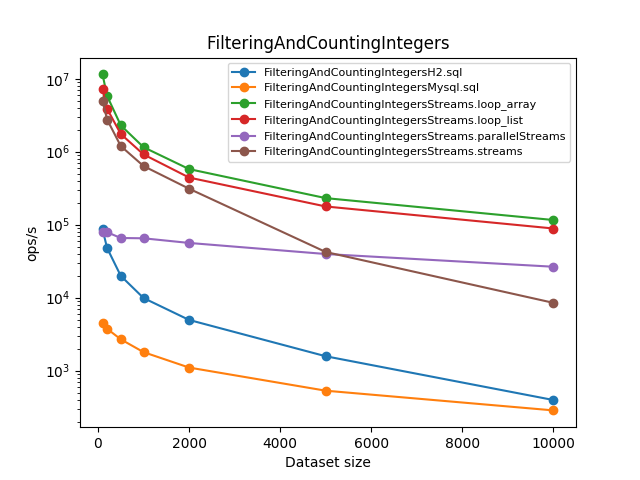
\includegraphics[width=13cm]{plots/FilteringAndCountingIntegers}
\caption{FilteringAndCountingIntegers}
\end{figure}

\begin{figure}[H]
\centering
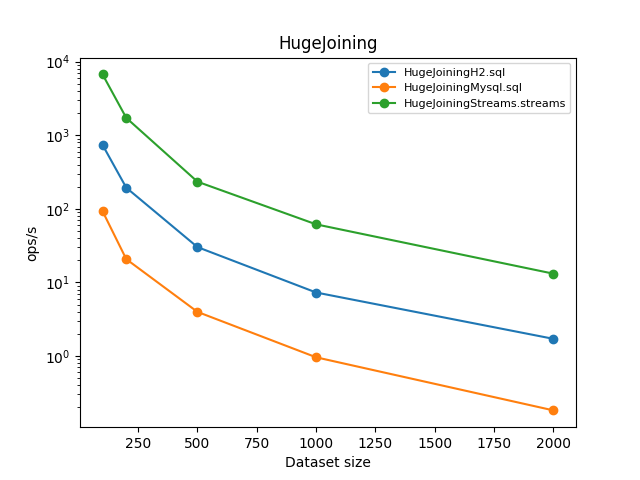
\includegraphics[width=13cm]{plots/HugeJoining}
\caption{HugeJoining}
\end{figure}




\subsection{Zbiór danych TPC-H} \label{tpc}

    TPC-H jest testem referencyjnym stworzonym przez organizację non-profit Transaction Processing Performance Council stosowanym do badania wydajności i profilowania silników bazodanowych. Składa się on z dwóch części: generatora danych testowych oraz zbioru zapytań.

    Generator danych testowych \texttt{dbgen} jest konsolowym programem, służącym do generowania zbiorów danych testowych TPC-H. Schemat bazy danych zaprezentowany jest na rysunku \ref{fig:tpcschema}. Jest to typowa hurtownia danych, gromadząca informacje o produktach, klientach, dostawcach i zamówieniach. Dokładny sens biznesowy wygenerowanych danych nie jest specjalnie istotny w rozważaniach wydajnościowych, na potrzeby niniejszej pracy zakłada się ich poprawność w sensie zgodności referencyjnej i reprezentatywności sytuacji możliwej do zaistnienia w rzeczywistości. Program \texttt{dbgen} pozwala na zdefiniowanie wielkości wygenerowanego zbioru, procentowo względem zbioru referencyjnego o wielkości 1.0. Ze względu na praktyczne ograniczenia platformy testowej, konieczne było ograniczenie maksymalnej wielkości zbioru do ok. 30\%, zależnie od przypadku testowego. 

    Drugą częścią TPC jest zbiór 22 zapytań testowych, które odpowiadają na pytania biznesowe i w rezultacje pomagają wspierać decyzje. Różnią się one znacznie stopniem skomplikowania (pod względem ogólnej złożoności kodu SQL) i średnim czasem wykonania. Prawidłowe wyniki wzorcowe są także udostępniane przez TPC, niestety jedynie dla zbioru danych o wielkości 1.0. Część zapytań można jednak zwalidować mimo tego, jeśli bazują one na typowych agregacjach typu suma, średnia czy ilość. Nie jest to oczywiście zbyt pewny sposób, tak więc do środowiska badawczego wprowadzono zbiór testów jednostkowych, które sprawdzają, czy wyniki uzyskane z wykonania zapytania na wszystkich systemach bazodanowych są identyczne.


\begin{figure}
\centering
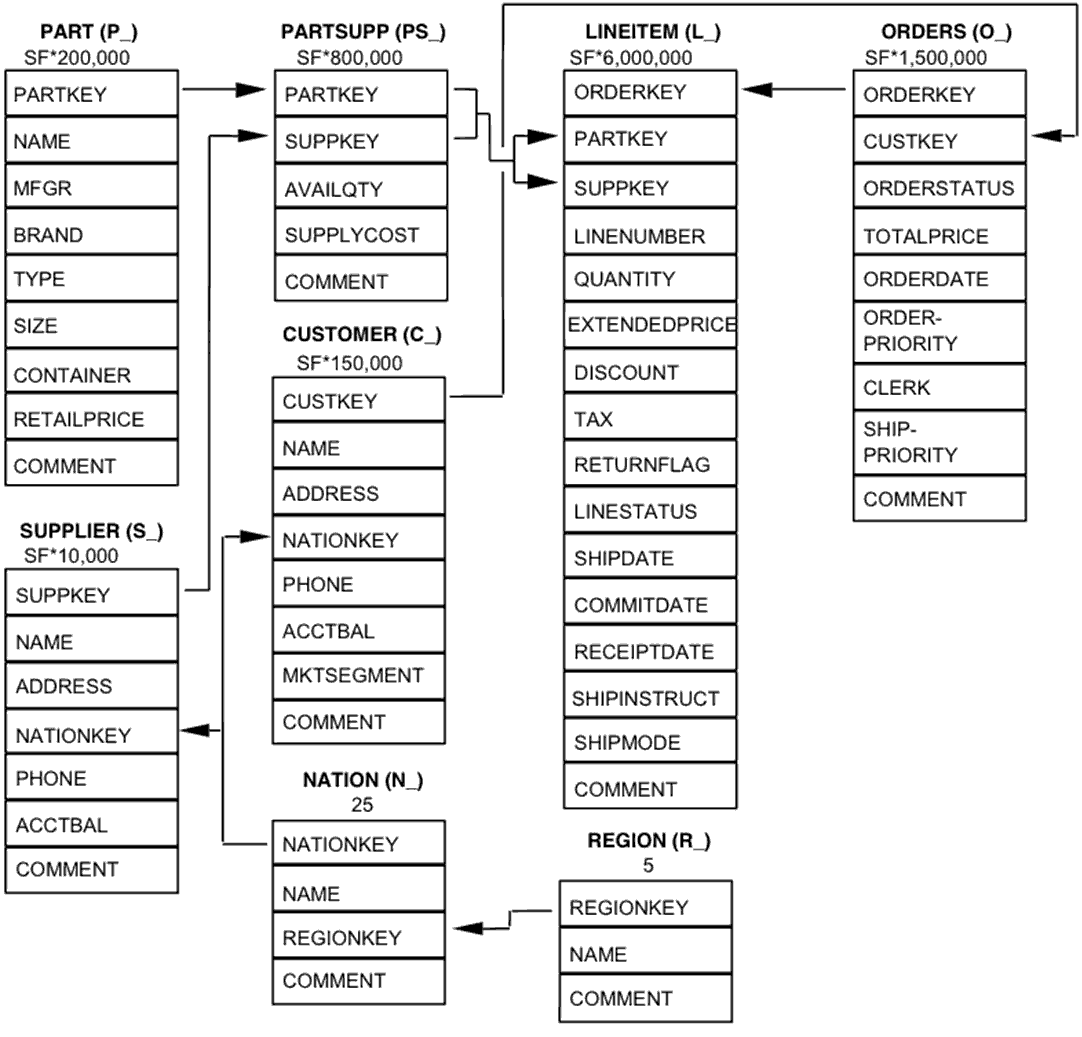
\includegraphics[width=11cm]{tpc-schema.png}
\caption{Schemat bazy danych TPC-H}
\label{fig:tpcschema}
\end{figure}

    Dokumentacja TPC-H definiuje 22 zapytania. Są to zapytania typowo statystyczne, pozwalające na ocenienie opłacalności pewnych biznesowych decyzji. Każde zapytanie określone jest przez problem biznesowy (kontekst), definicję zapytania SQL w standardzie SQL-92, parametry które należy podstawić oraz przewidywane wyniki.

\subsection{Odwzorowanie modelu TPC w języku Java}

    Aby umożliwić badanie działania strumieni na danych testu TPC, konieczne jest przekształcenie relacyjnego modelu danych w model, który jest możliwy do zareprezentowania w języku Java. Typowe odwzorowanie stosowane w systemach obiektowo-relacyjnych wykorzystuje pola obiektów do reprezentacji kolumn oraz referencje do obiektów do reprezentacji powiązań (kluczy obcych) pomiędzy tabelami. Zastosowano więc powyższy sposób do odwzorowania oryginalnej struktury. W rezultacje wynikowy model obiektowy jest bardzo podobny do modelu relacyjnego. Jedyną różnicą jest powiązanie kolekcji \texttt{Partsupp} z kolekcją \texttt{Lineitem} - zbiory te posiadają klucz główny będący kombinacją dwóch pól. Ze względu na dość powolny proces importu danych i budowania kolekcji, konieczne stało się dodanie do klasy \texttt{Partsupp} nowego pola, będącego złączeniem powyższych dwóch pól. Poza procesem wczytywania danych, złączony klucz główny nie jest wykorzystywany.

    Cała hutrownia danych reprezentowana jest przez obiekt klasy \texttt{Store}, który przechowuje wszystkie kolekcje danych TPC. Przy implementacji importu danych okazało się, że nie ma praktycznej możliwości wykorzystania zwykłych list jako kontenerów danych. Odczyt był bardzo powolny, w związku z tym zdecydowano się w większości miejsc na wykorzystanie kolekcji haszującej \texttt{HashMap}, w której jako klucze wykorzystano klucze główne obiektów, ze względu na ich unikalność. Z drugiej strony, nie wykorzystuje się właściwości haszujących przy badaniu wydajności strumieni, ponieważ założeniem jest, by właściwości strumieni były badane w izolacji, bez wpływu wykorzystanych struktur danych.

    * UML :)



\subsection{Wyniki badań dla danych TPC}

\begin{figure}[H]
\centering
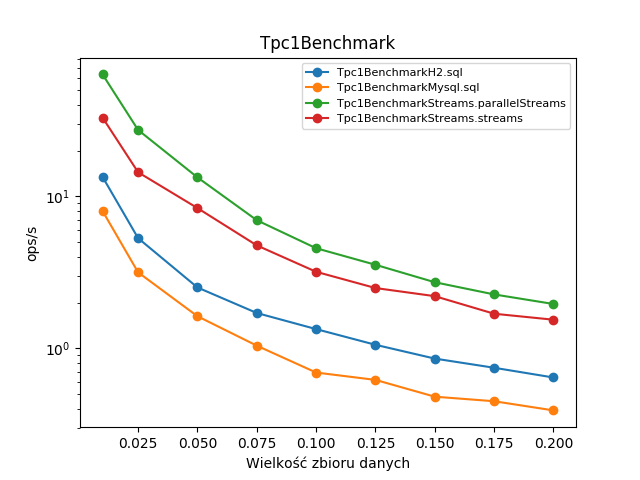
\includegraphics[width=13cm]{plots/Tpc1Benchmark}
\caption{Tpc1Benchmark}
\end{figure}

\begin{figure}[H]
\centering
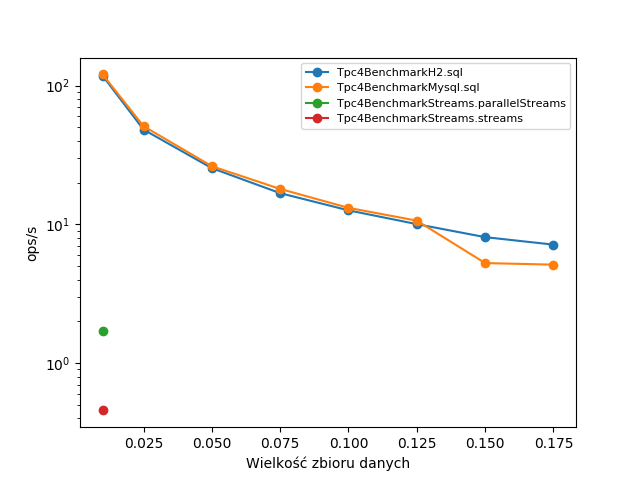
\includegraphics[width=13cm]{plots/Tpc4Benchmark}
\caption{Tpc4Benchmark}
\end{figure}

\begin{figure}[H]
\centering
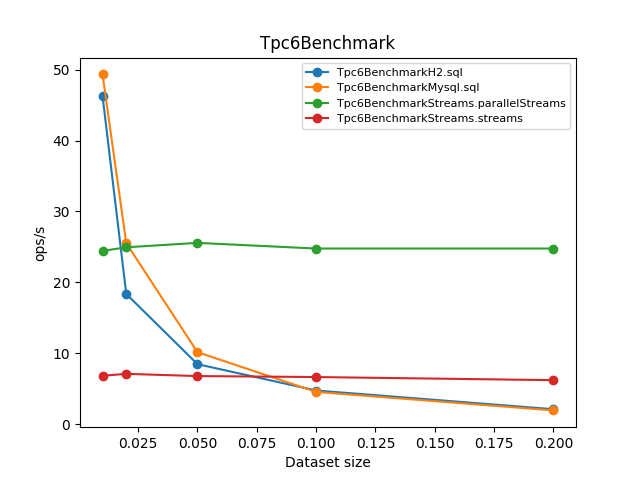
\includegraphics[width=13cm]{plots/Tpc6Benchmark}
\caption{Tpc6Benchmark}
\end{figure}

\begin{figure}[H]
\centering
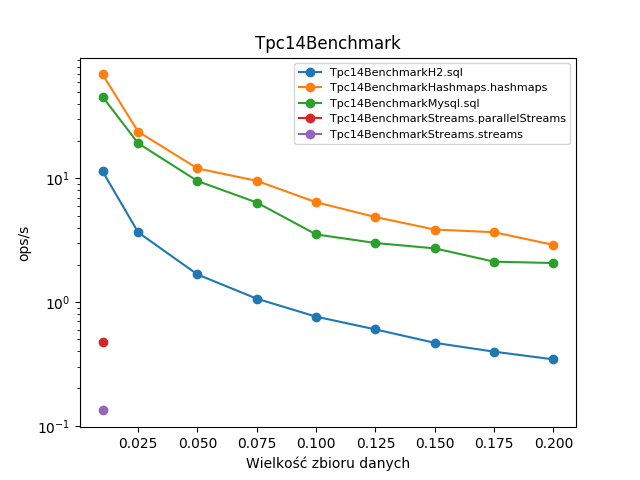
\includegraphics[width=13cm]{plots/Tpc14Benchmark}
\caption{Tpc14Benchmark}
\end{figure}

\subsection{Dodatek: Porównanie zajętości pamięci}

    W ramach badania wydajności metod dostępu do danych postanowiono dodatkowo sprawdzić ilość pamięci, wykorzystywanej przez bazy danych do ich przechowywania. Jak przewidywano, baza dyskowa MySQL przechowuje dane na dysku w najbardziej bardziej kompaktowej postaci. Schemat TPC w postaci obiektów znajdujących się w pamięci maszyny wirtualnej zajmuje więcej miejsca, natomiast w przypadku bazy pamięciowej H2 zaobserwować można pewien narzut wewnętrznych struktur danych.

\begin{figure}[H]
\centering
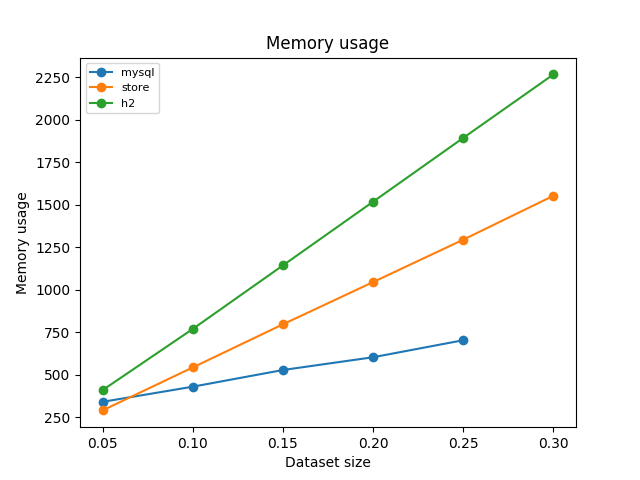
\includegraphics[width=13cm]{plots/memory}
\caption{Tpc14Benchmark}
\end{figure}
    


\section{Porównanie sposobu formułowania kodu}

\subsection{Proces wykonywania zapytania SQL}

    Jedną z ważniejszych cech języka programowania jest sposób interpretacji kodu programu przez interpreter bądź kompilator. Język SQL jest dość ciekawym przypadkiem, ponieważ leksykalna kolejność operacji jest odmienna od logicznej kolejności. Wprowadza to wiele zamieszania, zwłaszcza pośród początkujących programistów. Fragment \ref{sqlorder} prezentuje jprzykładowe zapytanie SQL, przeznaczone do wykonania na testowej bazie TPC:


\begin{lstlisting}[label=sqlorder, caption=Przykład kolejności wykonywania zapytania SQL]
select customers.name, sum(order.totalprice)
from orders 
    join customers on customers.custkey = orders.custkey
where customer.acctbal > 1000
group by customers.custkey, customers.name
having count(*) > 10
order by customers.name;
\end{lstlisting}

Pomijając bardzo prawdopodobne optymalizacje, powyższe zapytanie interpretowane jest w następujący sposób, w następującej kolejności:

\begin{itemize}
    \item \textbf{from orders join customer} - pierwszym krokiem jest wybranie tabeli (tabel), z których pobrane zostaną dane. Należy zauważyć, że klauzula \textbf{join} jest logicznie częścią klauzuli \textbf{where}, jedynie skrótowo zapisaną.
    \item \textbf{where customer.acctbal > 1000} - następnie wiersze są filtrowane. W tym momencie następuje odrzucenie niechcianych danych. 
    \item \textbf{group by customers.custkey, customers.name} - następuje tworzenie grup na podstawie podanej krotki. Podczas grupowania obliczane są wszystkie funkcje agregujące występujące w zapytaniu.
    \item \textbf{having count(*) > 10} - na grupach wykonywane jest dalsze filtrowanie, na podstawie wyliczonych w poprzednim kroku funkcji, tutaj sprawdzana jest wielkość grup.
    \item \textbf{select customers.name, sum(order.totalprice)} - z pośredniej tabeli, zawierającej jak dotąd wszystkie kolumny z obu tabel po połączeniu, wybierane są jedynie wymagane kolumny.
    \item \textbf{order by customers.name} - na samym końcu wykonywane jest sortowanie.
\end{itemize}

Jak można zauważyć, logiczna kolejność wykonywania zapytania jest znacząco odmienna od faktycznej kolejności.

\subsection{Proces wykonywania zapytania strumieniowego}

    Podobnie jak w przypadku języka SQL, zapytanie strumieniowe wykonuje się w kilku etapach. Ważną różnicą jest to, że nie występuje tutaj żaden mechanizm parsowania i tłumaczenia kodu, ponieważ zwykły kod języka Java jest już skompilowany do kodu bajtowego i wykonywany na maszynie wirtualnej Java. Maszyna wirtualna Javy po uruchomieniu programu realizuje dużą liczbę optymalizacji kodu, więc możliwe jest uzyskanie wzrostu wydajności jedynie dzięki tym optymalizacjom.
    Strumień, będąc abstrakcyjną formą reprezentacji źródła danych, tworzony może być na kilka różnych sposobów, ale sposoby te nie wpływają semantycznie na proces przetwarzania danych. Zwykle strumień tworzony jest na podstawie kolekcji - przy konsumowaniu elementów, kolekcja dostarcza elementy wykonując wewnętrzną iterację (internal iteration), która jest procesem ukrytym przed programistą. Inne sposoby tworzenia strumieni, takie jak generowanie ich w locie, wczytywanie z dysku bądź z sieci nie są zbyt przydatne z powodu ich konstrukcji pull-based. Decyzją implementacyjną projektantów Stream API było wykorzystanie modelu przetwarzania ciągłego, w którym to strumień wykonuje akcję pobrania następnego elementu. W związku z tym, nie jest możliwe (przynajmniej w domyślnej formie) efektywne asynchroniczne dostarczanie nowych elementów, ponieważ każda operacja pobrania elementu jest operacją blokującą, wywoływaną po zakończeniu przetwarzania poprzedniego elementu. Model odwrotny (push-based), wykorzystywany np. w bibliotekach RxJava bazujących na wzorcu Observable, ma lepsze zastosowanie w takich przypadkach.
    Po utworzeniu strumienia możliwe jest wykonanie dostępnych na nim operacji pośrednich, udostępnionych przez metody instancyjne klasy \texttt{Stream<T>}. Każda taka operacja zwraca zawsze strumień, ewentualnie innego typu (\texttt{Stream<...>}, \texttt{IntStream}). Należy zwrócić szczególną uwagę na różnice pomiędzy dwoma typami operacji pośrednich, ponieważ owe typy determinują faktyczną, wewnętrzną kolejność operacji, która mimo iż ukryta przed programistą, może mieć wpływ na złożoność czasową jak i pamięciową. Operacje pośrednie bezstanowe (takie jak \texttt{filter} i \texttt{map}) zapisane tuż obok siebie, łączone są w jedną, większą operację, wykorzystując właściwości kompozycji funkcji bezstanowych. Drugi typ operacji pośrednich, operacje pośrednie stanowe, nie gwarantują fuzji i mogą wprowadzać ukryty stan. Najlepszym przykładem operacji pośredniej stanowej jest sortowanie, które wymaga, aby dokładnie wszystkie elementy strumienia zbuforowane zostały przed sortowaniem. Jest to logiczne, ponieważ nie jest możliwe ustalenie posortowanej kolejności zbioru elementów o nieznanej wielkości. Przykład fuzji operacji zaprezentowany jest we fragmencie kodu \ref{streamstateful1}.

\begin{lstlisting}[label=streamstateful1, caption=Fuzja operacji bezstanowych]
Stream.of(1, 2, 3, 4, 5)
    .map(e -> {
      out.println("Mapping: " + e);
      return e;
    })
    .filter(e -> {
      out.println("Filtering: " + e);
      return true;
    })
    .sorted()
    .collect(toList());

\end{lstlisting}


\begin{verbatim}

Mapping: 1
Filtering: 1
Mapping: 2
Filtering: 2
Mapping: 3
Filtering: 3
Mapping: 4
Filtering: 4
Mapping: 5
Filtering: 5

\end{verbatim}

    Na podstawie wyjścia programu można stwierdzić, że operacja \texttt{map} wykonywała się wraz z operacją \texttt{filter}. Jako iż sortowanie zostało umieszczone na końcu, nie przeszkadzało ono w żaden sposób. Z drugiej strony, jeśli sortowanie zostanie przeniesione pomiędzy, można zaobserwować buforowanie się elementów tuż przed stanową operacją sortowania (fragment \ref{streamstateful2}).

\begin{lstlisting}[label=streamstateful2, caption=Brak fuzji operacji stanowych]
Stream.of(1, 2, 3, 4, 5)
    .map(e -> {
      out.println("Mapping: " + e);
      return e;
    })
    .sorted()
    .filter(e -> {
      out.println("Filtering: " + e);
      return true;
    })
    .collect(toList());
\end{lstlisting}

\begin{verbatim}

Mapping: 1
Mapping: 2
Mapping: 3
Mapping: 4
Mapping: 5
Filtering: 1
Filtering: 2
Filtering: 3
Filtering: 4
Filtering: 5

\end{verbatim}

    Ostatnim krokiem wykonywania się zapytania strumieniowego jest wykonanie operacji terminalnej, która wyznacza ostateczny wynik zapytania. Wystąpienie takiej operacji powoduje wykonanie wszystkich operacji pośrednich. 

* różnice parallel i sequential
* operacje terminalne i nieterminalne (typ zwracany), streams cannot be reused
* streamy są bardzo ograniczone, ale istnieją lepsze jooq streamex
* porównanie push-pull (Observable), streamy nie są async mimo parallell

\subsection{Ocena i krytyka}

    Wprowadzenie do języka Java mechanizmów programowania funkcyjnego zostało bardzo pozytywnie ocenione przez programistów, mimo iż mechanizmy te obecne były w innych językach programowania ogólnego przeznaczenia znacznie wcześniej. Duży nacisk projektantów platformy na wsteczną kompatybilność i obawy przed wprowadzeniem zmian, które nie okażą się korzystne, a konieczne będzie ich utrzymywanie, powodują, że język ten nie rozwija się w takim tempie, jak inne języki. Przykładowo, postanowiono nie wprowadzać metody \texttt{Iterable.stream} konwertującej obiekt wspierający protokół iteracji Java na strumień, mimo iż nie można wskazać żadnych przeciwwskazań do jej istnienia, a i można wskazać zastępcze rozwiązania, które mogłyby być wprowadzone bez większych zmian do API.

    Jednym z najczęściej występujących zarzutów odnośnie Stream API jest brak odpowiedzi na istniejące w języku C\# i platformie .NET narzędzie LINQ-to-SQL. Pozwala ono na dostęp do danych znajdujących się w bazie relacyjnej za pomocą specjalniej składni kodu C\#, z automatycznym odwzorowaniem typu ORM. Strumienie umożliwiają tworzenie dość złożonych kombinacji operacji, natomiast wszystkie te operacje zachodzą w pamięci maszyny wirtualnej. Nie jest możliwe tłumaczenie metod klasy \texttt{Stream} na słowa kluczowe zapytania SQL. Taką możliwość dają dodatkowe biblioteki, np. JOOQ bądź Hibernate Criteria API, ale dostępne one były jeszcze przed wydaniem Java 8. 

    Kolejnym argumentem przemiawiającym na niekorzyść strumieni jest obiektywnie niewielka liczba operacji możliwych do wykonywania na strumieniach. Podstawowe operacje znane z języków funkcyjnych są oczywiście dostępne, natomiast postanowiono celowo nie rozszerzać zbytnio API klasy \texttt{Stream}, aby nie spowodować bałaganu. Znaczy to, iż popularne operatory funkcyjne, znane z innych języków programowania, takie jak \texttt{takeWhile}, \texttt{zip} czy \texttt{sliding} nie są dostępne i nie będą w natywnej formie, ponieważ nie jest możliwe modyfikowanie klas języka Java bez tworzenia własnych klas pośredniczących. Istnieją co prawda biblioteki takie jak jOOQlambda czy StreamEx, dostarczające dodatkowe funkcjonalności, ale nie są one oficjalne i nie posiadają wsparcia ze strony języka. W nowej wersji języka, Java 9, zapowiedziano wprowadzenie kilku dodatkowych operatorów, ale nie jest to nadal to samo.


\section{Propozycje rozwiązań}

\subsection{Strumieniowy operator złączenia}

    Jedną z najczęściej wykonywanych operacji na relacyjnej bazie danych jest łączenie tabel. W języku SQL dostępne są różne typy złączeń (\texttt{JOIN}, \texttt{INNER JOIN}, \texttt{LEFT/RIGHT JOIN} i inne), które wykorzystywane są w różnych sytuacjach. Relacyjne bazy danych posiadają z reguły znaczne optymalizacje w zakresie wykonywania takich operacji, ponieważ wykorzystywane są one bardzo często - ważną zaletą modelu relacyjnego jest podział na tabele połączone ze sobą kluczami i więzami referencyjnymi. Aby osiągnąć wymaganą wydajność, w większości rozwiązań kolumny będące kluczami głównymi otrzymują automatycznie, przy ich tworzeniu, indeks.
    TODO coś o indeksach

    Ze względu na porównawczy charakter niniejszej pracy, zdecydowano się na opracowanie podobnego rozwiązania, działającego w oparciu o Stream API. Problem zdefiniowany został następująco

\begin{theorem}
    Dane są dwie kolekcje typów \texttt{T} i \texttt{U} o rozmiarach $ n $ i $ m $. Należy zaproponować rozwiązanie, pozwalające na złączenie tych kolekcji na podstawie warunku równości dowolnych kluczy, będących właściwościami obiektów, bądź funkcjami właściwości obiektów. Wynik powinien dany być listą par \texttt{(T, U)}.
\end{theorem}

    Pierwsze rozwiązanie, najbardziej intuicyjne, polega utworzeniu wszystkich możliwych par \texttt{(T, U)} i odfiltrowaniu pasujących. Do tego celu wykorzystano metodę \texttt{Stream.flatMap}, która dla każdego obiektu strumienia tworzy nowy strumień nań bazujący, a następnie łączy wszystkie pośrednie strumienie w jeden.

\begin{lstlisting}[label=join1, caption=Rozwiązanie nr 1]

public static <T, U> Stream<ImmutablePair<T, U>>
innerJoin(
    Collection<T> first,
    Collection<U> second,
    Predicate<ImmutablePair<T, U>> condition
) {
  return first.stream().flatMap(firstItem ->
      second.stream().map(secondItem ->
          new ImmutablePair<>(firstItem, secondItem)
      )
  ).filter(condition);
}

\end{lstlisting}

    Rozwiązanie to, mimo iż krótkie i czytelne, wykazuje się bardzo niekorzystną złożonością obliczeniową, i w konsekwencji, bardzo słabą wydajnością. Ze względu na konieczność utworzenia $ mn $ par niezależnie od przypadku, aktywność GC jest znaczna, ponieważ mnóstwo obiektów tworzonych jest tylko w celu ich odśmiecenia.

    Rozwiązanie drugie polega na przepisaniu strumieniowej części w postaci zwykłej pętli. Strumienie mają nieznaczny narzut czasowy i pamięciowy, więc warto sprawdzić, czy możliwe jest jego uniknięcie.

\begin{lstlisting}[label=join2, caption=Rozwiązanie nr 2]

public static <T, U> Stream<ImmutablePair<T, U>>
innerJoinForLoop(
    Collection<T> first,
    Collection<U> second,
    BiPredicate<T, U> condition
) {
  List<ImmutablePair<T, U>> result = new ArrayList<>();
  for (T t : first) {
    for (U u : second) {
      if (condition.test(t, u)) {
        result.add(new ImmutablePair<>(t, u));
      }
    }
  }
  return result.stream();
    

\end{lstlisting}

    To rozwiązanie jest nieco lepsze, natomiast nie jest znacząco lepsze od poprzedniego. Problemem jest konieczność przejścia przez wewnętrzną pętlę nadal $ mn $ razy.

    W rozwiązaniu trzecim postanowiono wykorzystać kolekcje haszujące, które spełniają w nim rolę podobną do indeksów. Przy założeniu, że kolekcje łączone są warunkiem równości właściwości, z których co najmniej jedna spełnia właściwości klucza głównego (unikalność i brak występowania wartości pustej \texttt{NULL}), możliwe jest umieszczenie elementów tej kolekcji w strukturze mapy haszującej, w której za klucz przyjmuje się wymieniony klucz główny, a za wartość - obiekt przez ten klucz reprezentowany. Dzięki temu, nie jest wymagane przeglądanie całej kolekcji elementów \texttt{T}, a jedynie sprawdzenie, czy obiekt identyfikowany przez kolejne obiekty kolekcji \texttt{U} istnieje bądź nie.

\begin{lstlisting}[label=join3, caption=Rozwiązanie nr 3]

public static <T, U> Stream<ImmutablePair<T, U>> innerJoinHashmaps(
    Collection<T> left,
    Function<T, Object> leftKeyExtractor,
    Collection<U> right,
    Function<U, Object> rightKeyExtractor
) {
  HashMap<Object, T> leftMap = new HashMap<>();
  for (T leftElement : left) {
    leftMap.put(
      leftKeyExtractor.apply(leftElement),
      leftElement
    );
  }
  
  List<ImmutablePair<T, U>> result = new ArrayList<>();
  
  for (U rightElement : right) {
    T leftElement = leftMap.get(
      rightKeyExtractor.apply(rightElement)
    );
    if (leftElement != null) {
      result.add(new ImmutablePair<>(
        leftElement, rightElement
      ));
    }
  }
  
  return result.stream();
}
\end{lstlisting}

Rozwiązanie to jest znacznie szybsze, wymaga jednak unikalności wartości klucza w jednej z kolekcji. Porównanie szybkości wykonywania się operacji złączenia na zbiorze danych TPC jest poniżej.


\begin{figure}[H]
\centering
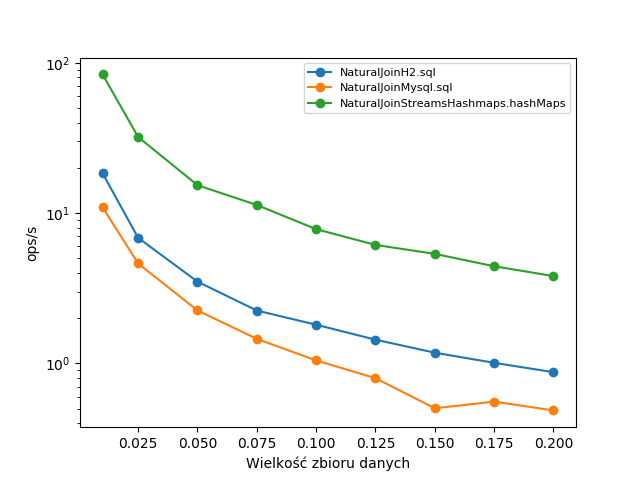
\includegraphics[width=13cm]{plots/NaturalJoin}
\caption{Porównanie wydajności złączenia naturalnego}
\end{figure}

\begin{thebibliography}{9}
\bibitem{latexcompanion} 
Raoul-Gabriel Urma
\textit{Processing Data with Java SE 8 Streams, Part 1}. 
http://www.oracle.com/technetwork/articles/java/ma14-java-se-8-streams-2177646.html, czas dostępu 26.05.2017
 
\end{thebibliography}

\end{document}
